\chapter{Literature Review}

In order to get an understanding of the concepts and best practices in the field of vascular biometrics, it is important to review the available literature on the topic.




%\begin{figure}[ht]
%\centering
%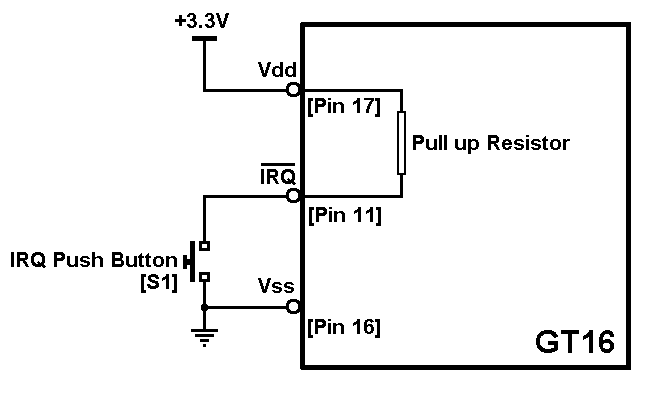
\includegraphics[width=0.7\textwidth]{model.png}
%\caption{A block diagram illustrating the connections to the IRQ pin on the MCS08GT16A microcontroller (Please
%note that your headings should be short descriptions of what is in the diagram not simply the figure title)}
%\label{fig:model}
%\end{figure}


\section{Biometrics as a Verification Technique}

Over the past few decades there has been a gradual shift into the virtual domain. As more people go online there becomes a greater incentive for companies to provide online services. However this expansion into the digital domain comes at a cost. As individuals add more and more services to their virtual network they become bogged down in keeping up with passwords. While a common method is to use the same password for all your online accounts this is usually not recommended because a vulnerability in one service can compromise the entire system. This can be even more detrimental if the password is also associated with a banking service.






